\documentclass[xetex,mathserif,serif]{beamer}

\usepackage{mathspec}
\usepackage{xltxtra,fontspec,xunicode}
\usepackage{listings}

% \usepackage{pgfpages}
% \pgfpagesuselayout{4 on 1}[a4paper,border shrink=5mm,landscape]

% Features
\setbeamertemplate{navigation symbols}{}

% Fonts
\setmainfont{Helvetica}
\setmathsfont(Digits,Latin,Greek){Helvetica}
\setmonofont{Monaco}

% Macros
\definecolor{CodeColor}{RGB}{0,112,0}
\newcommand{\code}[1]{\mbox{\texttt{\small{\color{CodeColor}{#1}}}}}

\title{Faster persistent data structures through hashing}
\author{Johan Tibell\\johan.tibell@gmail.com}
\date{2011-09-23}

\begin{document}
\lstset{
  language=Haskell,
  basicstyle=\small\ttfamily,
  keywordstyle=,
  commentstyle=\color{CodeColor}}

\frame{\titlepage}

\begin{frame}
  \frametitle{Motivating problem: Twitter data analysis}

  \begin{quote}
    I'm computing a communication graph from Twitter data and then
    scan it daily to allocate social capital to nodes behaving in a
    good karmic manner.  The graph is culled from 100 million tweets
    and has about 3 million nodes.
  \end{quote}

  \bigskip
  We need a data structure that is
  \begin{itemize}
  \item fast when used with string keys, and
  \item doesn't use too much memory.
  \end{itemize}
\end{frame}

\begin{frame}
  \frametitle{Persistent maps in Haskell}

  \begin{itemize}
  \item \code{Data.Map} is the most commonly used map type.
  \item It's implemented using size balanced trees and is
    representative of the performance of other binary tree
    implementations.
  \item Keys can be of any type, as long as values of the type can be
    ordered.
  \end{itemize}
\end{frame}

\begin{frame}
  \frametitle{Real world performance of Data.Map}

  \begin{itemize}
  \item Good in theory: no more than $O(\log n)$ comparisons.
  \item Not great in practice: up to $O(\log n)$ comparisons!
  \item Many common types are expensive to compare e.g
    \code{String}, \code{ByteString}, and \code{Text}.
  \item Given a string of length $k$, we need $O(k*\log n)$
    comparisons to look up an entry.
  \end{itemize}
\end{frame}

\begin{frame}
  \frametitle{Hash tables}
  \begin{itemize}
  \item Hash tables perform well with string keys: $O(k)$ amortized
    lookup time for strings of length $k$.
  \item However, we want persistent maps, not mutable hash tables.
  \end{itemize}
\end{frame}

\begin{frame}[fragile]
  \frametitle{Milan Straka's idea: IntMaps as arrays}
  \begin{itemize}
  \item We can use hashing without using hash tables!
  \item \code{Data.IntMap} implements a persistent array and is much
    faster than \code{Data.Map}.
  \item Use hashing to derive an \code{Int} from an arbitrary
    key.
  \end{itemize}
  \begin{lstlisting}
    class Hashable a where
      hash :: a -> Int
  \end{lstlisting}
\end{frame}

\begin{frame}
  \frametitle{Collisions are easy to deal with}
  \begin{itemize}
  \item \code{IntMap} implements a sparse, persistent array of size
    $2^{32}$ (or $2^{64}$).
  \item Hashing using this many buckets makes collisions rare: for
    $2^{24}$ entries we expect about 32,000 single collisions.
  \item Implication: We can use any old collision handling strategy
    (e.g. chaining using linked lists).
  \end{itemize}
\end{frame}

\begin{frame}[fragile]
  \frametitle{HashMap implemented using an IntMap}

  Naive implementation:

  \begin{lstlisting}
    newtype HashMap k v = HashMap (IntMap [(k, v)])
  \end{lstlisting}

  By inlining (``unpacking'') the list and pair constructors we can
  save 2 words of memory per key/value pair.
\end{frame}

\begin{frame}
  \frametitle{Benchmark: Map vs HashMap}

  Keys: $2^{12}$ random 8-byte \code{ByteString}s

  \bigskip
  \begin{center}
  \begin{tabular}{r|rrr}
                  & \multicolumn{2}{c}{Runtime ($\mu$s)} & Runtime \\
                  & Map & HashMap & \% increase \\
    \hline lookup & 1956 &  916 & -53\% \\
           insert & 3543 & 1855 & -48\% \\
           delete & 3791 & 1838 & -52\% \\
  \end{tabular}
  \end{center}
\end{frame}

\begin{frame}
  \frametitle{Can we do better?}
  \begin{itemize}
  \item Imperative hash tables still perform better, perhaps there's
    room for improvement.
  \item We still need to perform $O(min(W, \log n))$ \code{Int}
    comparisons, where $W$ is the number of bits in a word.
  \item The memory overhead per key/value pair is still high, about 9
    words per key/value pair.
  \end{itemize}
\end{frame}

\begin{frame}
  \frametitle{Borrowing from our neighbours}
  \begin{itemize}
  \item Clojure uses a \emph{hash-array mapped trie} (HAMT) data
    structure to implement persistent maps.
  \item Described in the paper ``Ideal Hash Trees'' by Bagwell (2001).
  \item Originally a mutable data structure implemented in C++.
  \item Clojure's persistent version was created by Rich Hickey.
  \end{itemize}
\end{frame}

\begin{frame}
  \frametitle{Hash-array mapped tries}
  \begin{itemize}
  \item Shallow tree with high branching factor.
  \item Each node, except the leaf nodes, contains an array of up to
    32 elements.
  \item 5 bits of the hash are used to index the array at each level.
  \item A clever trick, using bit population count, is used to
    represent sparse arrays.
  \end{itemize}
\end{frame}

\begin{frame}
  \frametitle{HAMT}
  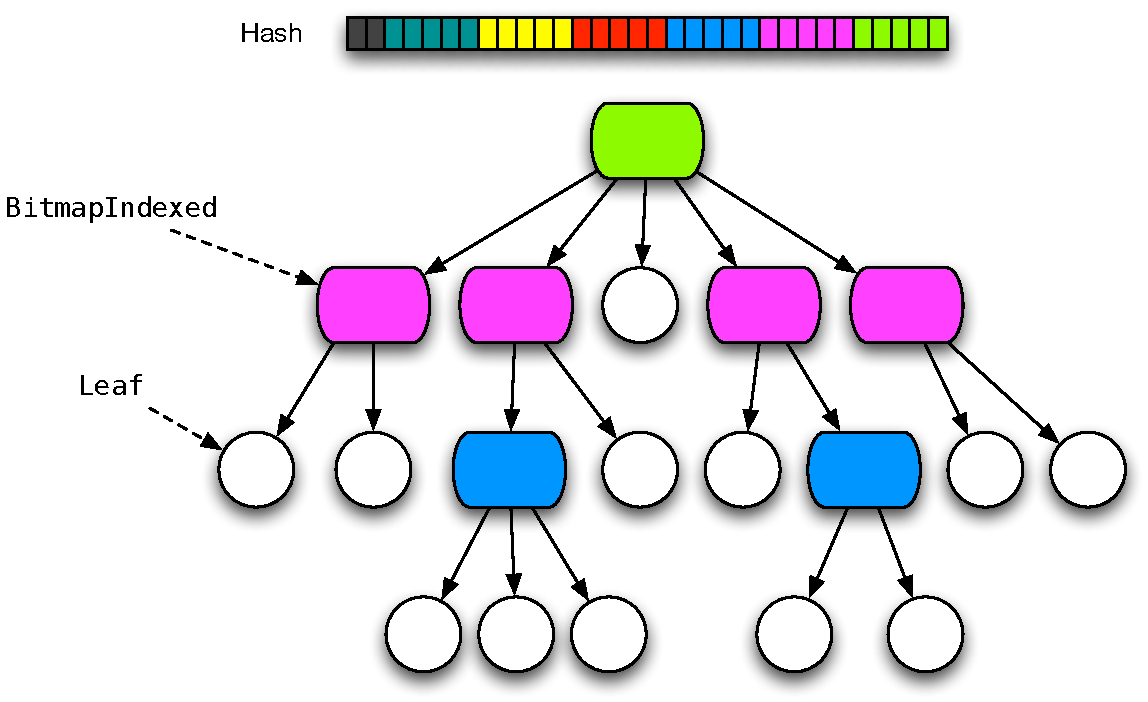
\includegraphics[width=\textwidth]{hamt.pdf}
\end{frame}


\begin{frame}[fragile]
  \frametitle{The Haskell definition of a HAMT}
  \begin{lstlisting}
data HashMap k v
    = Empty
    | BitmapIndexed !Bitmap !(Array (HashMap k v))
    | Leaf !Hash !k v
    | Full !(Array (HashMap k v))
    | Collision !Hash !(Array (Leaf k v))

type Bitmap = Word
type Hash = Int
data Array a = Array (Array# a)
  \end{lstlisting}
\end{frame}

\begin{frame}
  \frametitle{High performance Haskell programming}
  Optimized implementation using standard techniques:
  \begin{itemize}
  \item constructor unpacking,
  \item GHC's new \code{INLINABLE} pragma, and
  \item paying careful attention to strictness.
  \end{itemize}
  \code{insert} performance still bad (e.g compare to hash tables).
\end{frame}

\begin{frame}
  \frametitle{Optimizing insertion}

  \begin{itemize}
  \item Most time in \code{insert} is spent copying small arrays.
  \item Array copying is implemented in Haskell and GHC doesn't apply
    enough loop optimizations to make it run fast.
  \item When allocating arrays GHC fills the array with dummy
    elements, which are immediately overwritten.
  \end{itemize}
\end{frame}

\begin{frame}
  \frametitle{Optimizing insertion: copy less}

  \begin{itemize}
  \item Bagwell's original formulation used a fanout of 32.
  \item A fanout of 16 seems to provide a better trade-off between
    \code{lookup} and \code{insert} performance in our setting.
  \item Improved performance by 14\%
  \end{itemize}
\end{frame}

\begin{frame}
  \frametitle{Optimizing insertion: copy faster}

  \begin{itemize}
  \item Daniel Peebles and I have implemented a set of new primops for
    copying arrays in GHC.
  \item The implementation generates straight-line code for copies of
    statically known small size, and uses a fast \code{memcpy}
    otherwise.
  \item Improved performance by 20\%
  \end{itemize}
\end{frame}

\begin{frame}
  \frametitle{Optimizing insertion: common patterns}
  \begin{itemize}
  \item In many cases maps are created in one go from a sequence of
    key/value pairs.
  \item We can optimize for this case by repeatedly mutating the HAMT
    and freezing it when we're done.
  \end{itemize}

  \bigskip
  Keys: $2^{12}$ random 8-byte \code{ByteString}s

  \bigskip
  \begin{center}
  \begin{tabular}{c|c}
                         & Runtime (\%) \\
    \hline fromList/pure & 100 \\
           fromList/mutating & 50 \\
  \end{tabular}
  \end{center}
\end{frame}

\begin{frame}
  \frametitle{Optimizing lookup: Faster population count}
  \begin{itemize}
  \item Tried several bit population count implementations.
  \item Best speed/memory-use trade-off is a lookup table based
    approach.
  \item Using the \code{POPCNT} SSE 4.2 instructions improves the
    performance of \code{lookup} by 12\%.
  \end{itemize}
\end{frame}

\begin{frame}
  \frametitle{Benchmark: IntMap-based vs HAMT}

  Keys: $2^{12}$ random 8-byte \code{ByteString}s

  \bigskip
  \begin{center}
  \begin{tabular}{r|rrr}
                  & \multicolumn{2}{c}{Runtime ($\mu$s)} & Runtime \\
                  & IntMap & HAMT                      & \% increase \\
    \hline lookup &  916 &  477 & -48\% \\
           insert & 1855 & 1998 & 8\% \\
           delete & 1838 & 2303 & 25\% \\
  \end{tabular}
  \end{center}

  The benchmarks don't include the \code{POPCNT} optimization, due to
  it not being available on many architectures.
\end{frame}

\begin{frame}
  \frametitle{Memory usage: IntMap-based}
  Total: 96 MB, tree: 66MB ($2^{20}$ \code{Int} entries)
  \begin{center}
  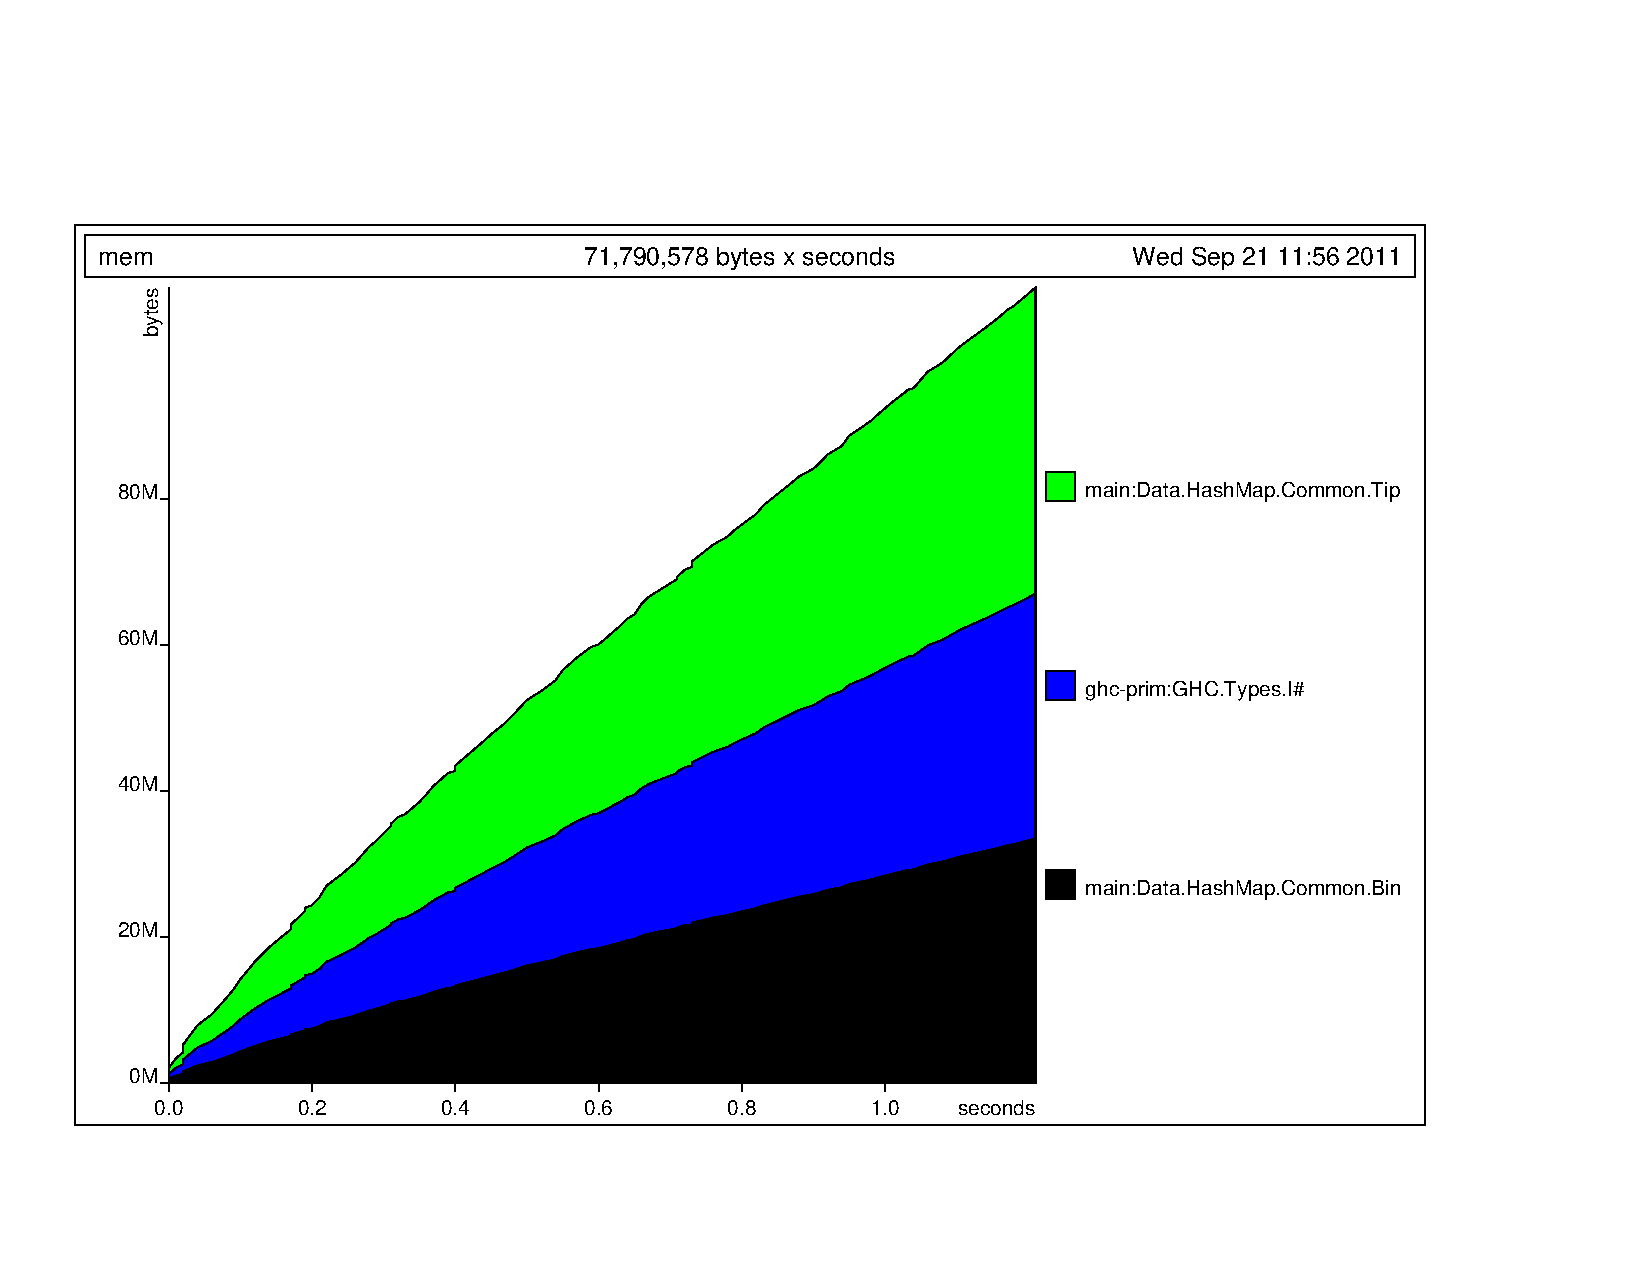
\includegraphics[angle=90,scale=0.3]{patricia-mem.pdf}
  \end{center}
\end{frame}

\begin{frame}
  \frametitle{Memory usage: HAMT}

  Total: 71MB, tree: 41MB ($2^{20}$ \code{Int} entries)
  \begin{center}
  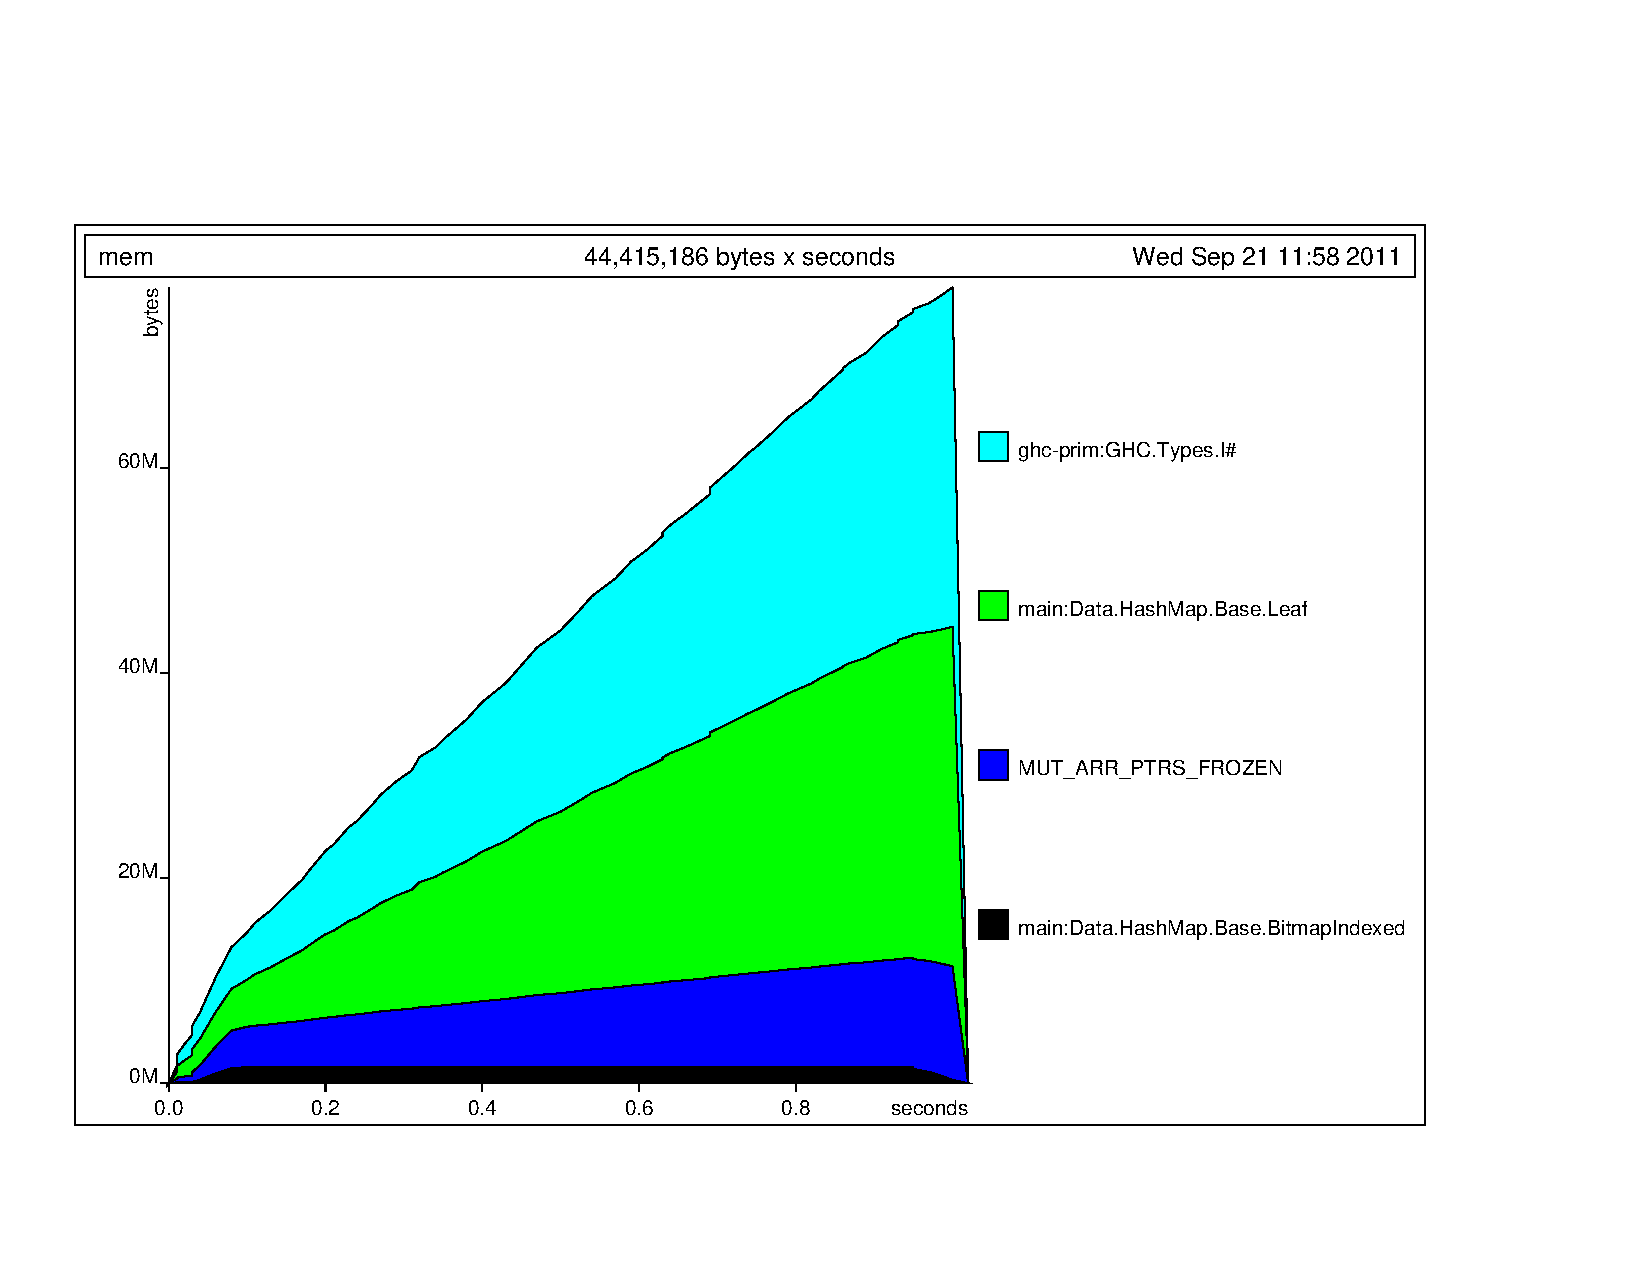
\includegraphics[angle=90,scale=0.3]{hamt-mem.pdf}
  \end{center}
\end{frame}

\begin{frame}
  \frametitle{Summary}
  Keys: $2^{12}$ random 8-byte \code{ByteString}s

  \bigskip
  \begin{center}
  \begin{tabular}{r|rrr}
                  & \multicolumn{2}{c}{Runtime ($\mu$s)} & Runtime \\
                  & Map & HAMT & \% increase \\
    \hline lookup & 1956 &  477 & -76\% \\
           insert & 3543 & 1998 & -44\% \\
           delete & 3791 & 2303 & -39\% \\
  \end{tabular}
  \end{center}
\end{frame}

\end{document}

%%% Local Variables:
%%% mode: latex
%%% TeX-master: t
%%% TeX-PDF-mode: t
%%% End:
